\newpage
\lecture{5}{Счётная аддитивность и субаддитивность.}

\subsection{Связи между понятиями.}

\begin{definition}
    Под \mdef{мерой} будем понимать конечно-аддитивные или счётно-аддитивные функции $\mu$, определенные хотя бы на
    полукольце такие, что $\mu(\varnothing)=0$.
\end{definition}

Проиллюстрируем некоторые базовые связи между данными определениями.

\begin{claim}
    \label{lect5:cl1}
    Пусть $\F\subset\CP(X)$~--- полукольцо и $\mu:\ \F\rightarrow[0,\,+\infty]$. Тогда
    \begin{enumerate}
        \item Если $\mu$~--- конечно-аддитивна, то $\mu$~--- монотонна и конечно-субаддитивна;
        \item Если $\mu$~--- $\sigma$"=аддитивна, то $\mu$~--- конечно-аддитивна и $\sigma$"=субаддитивна.
    \end{enumerate}

    \begin{remark}
        Если $\mu(\varnothing)>0$, то в силу конечной аддитивности $\forall A\in\F:$
        \[\mu(A)=\mu(A\sqcup \varnothing)=\mu(A)+\mu(\varnothing)\Rightarrow\mu(A)=+\infty,\]
        то есть $\mu\equiv +\infty$, но для такой тривиальной меры утверждение очевидно, поэтому далее не уменьшая общности
        считаем, что $\mu(\varnothing)=0$.
    \end{remark}

    \begin{proof}
        \begin{enumerate}
            \item Докажем монотонность. Пусть $A\subset B$~--- элементы $\F$. Так как $\F$~--- полукольцо, то $A$ можно дополнить до $B$ конечным набором элементов
                  полукольца: $\exists B_1,\,\ldots,\, B_n\in\F:\ B\setminus A = \bigsqcup\limits_{k=1}^n B_k$. Следовательно,
                  \[
                      \mu(B)=\mu\left(A\bigsqcup\left(\bigsqcup_{k=1}^n B_k\right)\right)=
                      \mu(A)+\sum_{k=1}^n\mu(B_k)\geqslant \mu(A).
                  \]

                  Теперь докажем конечную субаддитивность. Пусть $\bigcup\limits_{k=1}^n A_k\in\F$, где $A_k\in\F$.
                  Нужно доказать, что мера этого объединения меньше, чем сумма соответствующих мер. Возьмем
                  \[
                      B_k=A_k\setminus \underbrace{\bigcup_{l=1}^{k-1}A_l}_{\text{при $k=1:\varnothing$.}}
                  \]
                  Тогда $B_k\in\CR(\F)$, поэтому по теореме о структуре порожденного полукольцом кольца каждое $B_k$ выражается
                  как дизъюнктное объединение элементов полукольца: $B_k=\bigsqcup\limits_{l=1}^{N_k}P_{kl}$, где $P_{kl}\in\F$.
                  Поэтому
                  \begin{equation}
                      \mu\left(\bigcup_{k=1}^{n}A_k\right)=\mu\left(\bigsqcup_{k=1}^{n}B_k\right)=
                      \mu\left(\bigsqcup_{k=1}^n\bigsqcup_{l=1}^{N_k}P_{kl}\right)=
                      \sum_{k=1}^n\sum_{l=1}^{N_k}\mu(P_{kl}).
                      \label{eq:lect5:claim}
                  \end{equation}

                  Далее $A_k\setminus B_k\in\CR(\F)\Rightarrow A_k\setminus B_k=\bigsqcup\limits_{s=1}^{M_k}Q_{ks}$, где $Q_{ks}\in\F$. Тогда
                  \[
                      A_k=B_k\sqcup A_k\setminus B_k=\bigsqcup_{l=1}^{N_k}P_{kl}\sqcup\bigsqcup_{s=1}^{M_k}Q_{ks}.
                  \]
                  Теперь можем разложить меру $A_k$ в сумму:
                  \[
                      \mu(A_k)=\sum_{l=1}^{N_k}\mu(P_{kl})+\sum_{s=1}^{M_k}\underbrace{\mu(Q_{ks})}_{\geqslant 0}\geqslant\sum_{l=1}^{N_k}\mu(P_{kl}).
                  \]
                  Возвращаемся к уравнению \eqref{eq:lect5:claim}:
                  \[
                      \mu\left(\bigcup_{k=1}^{n}A_k\right)=
                      \sum_{k=1}^n\sum_{l=1}^{N_k}\mu(P_{kl})\leqslant
                      \sum_{k=1}^n\mu(A_k).
                  \]

            \item Докажем конечную аддитивность:
                  \[
                      \mu\left(\bigsqcup_{k=1}^n A_k\right)=\mu\left(\bigsqcup_{k=1}^n A_k\sqcup \bigsqcup_{k=n+1}^{\infty}\varnothing\right)=
                      \sum_{k=1}^n\mu(A_k)+\sum_{k=n+1}^{\infty}\mu(\varnothing)=\sum_{k=1}^n\mu(A_k).
                  \]
                  И не забываем про $\sigma$"=субаддитивность. Нужно доказать, что
                  \[
                      \mu\left(\bigcup_{k=1}^{\infty} A_k\right)\stackrel[]{?}{\leqslant}\sum_{k=1}^{\infty}\mu(A_k).
                  \]
                  Снова введем $B_k$ как в пункте 1:
                  \[
                      B_k=A_k\setminus\bigcup_{l=1}^{k-1}A_l=\bigsqcup_{l=1}^{N_k}P_{kl},\quad P_{kl}\in\F.
                  \]
                  Тогда имеем:
                  \[
                      \mu\left(\bigcup_{k=1}^{\infty}A_k\right)=\mu\left(\bigsqcup_{k=1}^{\infty}B_k\right)=\mu\left(\bigsqcup_{k=1}^{\infty}\bigsqcup_{l=1}^{N_k}
                      P_{kl}\right)=\sum_{k=1}^{\infty}\underbrace{\sum_{l=1}^{N_k}\mu(P_{kl})}_{\leqslant\mu(A_k)}.
                  \]
        \end{enumerate}

    \end{proof}
\end{claim}

\begin{remark}
    Пусть $A\subset \bigcup\limits_{k=1}^n A_k$, где $A,\, A_k\in\F$ и $\mu$~--- конечно-субаддитивна и монотонна (в частности, если
    конечно-аддитивна).
    Тогда \[\mu(A)\leqslant\sum_{k=1}^n\mu(A_k).\]

    \begin{proof}
        Заметим, что $A=\bigcup\limits_{k=1}^n\underbrace{\left(A\cap A_k\right)}_{\in\F}$, так как $\F$~--- полукольцо.
        Следовательно \[
            \mu(A)\leqslant\underbrace{\sum_{k=1}^n\mu(A\cap A_k)\leqslant\sum_{k=1}^n \mu(A_k)}_{\text{в силу монотонности}}.
        \]

    \end{proof}
\end{remark}

\begin{claim}
    \label{lect5:cl2}
    Пусть $\F\subset\CP(X)$~--- полукольцо, $\mu:\ \F\rightarrow[0,\,+\infty]$~--- конечно-аддитивна и $\sigma$"=субаддитивна. Тогда
    $\mu$~--- $\sigma$"=аддитивна.

    \begin{proof}
        Пусть $\bigsqcup\limits_{k=1}^{\infty}A_k\in\F$, где $A_k\in\F\ \forall k\in \N$.
        Тогда \[
            \forall n\in\N\ \exists P_1,\,\ldots,\, P_m:\ \bigsqcup\limits_{k=1}^{\infty}A_k=\bigsqcup\limits_{k=1}^{n}A_k\sqcup\bigsqcup
            \limits_{l=1}^{m}P_l.
        \]
        Тогда в силу конечной аддитивности:
        \[
            \mu\left(\bigsqcup_{k=1}^{\infty}A_k\right)=\sum_{k=1}^n\mu(A_k)+\sum_{l=1}^m \underbrace{\mu(P_l)}_{\geqslant 0}
            \geqslant \sum_{k=1}^n\mu(A_k).
        \]
        Так как неравенство выше доказано для произвольного $n\in\N$, переходя к пределу получаем:
        \[
            \mu\left(\bigsqcup_{k=1}^{\infty}A_k\right)\geqslant\sum_{k=1}^{\infty}\mu(A_k).
        \]
        Осталось доказать неравенство в другую сторону. В силу $\sigma$"=субаддитивности
        \[
            \mu\left(\bigsqcup_{k=1}^{\infty}A_k\right)\leqslant\sum_{k=1}^{\infty}\mu(A_k).
        \]

    \end{proof}
\end{claim}

\subsection{Клеточная мера.}

Напомним, что множество клеток~--- это множество всевозможных декартовых произведений конечных промежутков (смотри лекцию 1).

\begin{definition}
    Функция $m:\ K_d\rightarrow[0,\,+\infty]$ вида
    \[
        m(I_1\times I_2\times\ldots\times I_d) = m(I_1)\cdot m(I_2)\cdot\ldots\cdot m(I_d),
    \]
    где $m(I_k)=\sup I_k-\inf I_k$~--- <<длина>> $I_k$, называется \mdef{клеточной мерой}.
\end{definition}

\begin{figure}
    \centering
    \begin{minipage}{.4\textwidth}
        \centering
        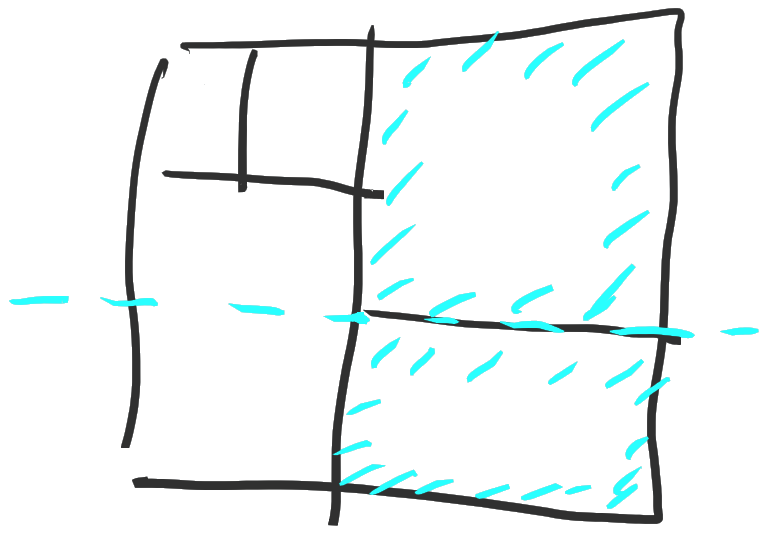
\includegraphics[width=0.7\linewidth]{lect5_1.png}
        \caption{К утверждению \ref{lect5:cl3}.}
        \label{fig:lect5:1}
    \end{minipage}%
    \begin{minipage}{.6\textwidth}
        \centering
        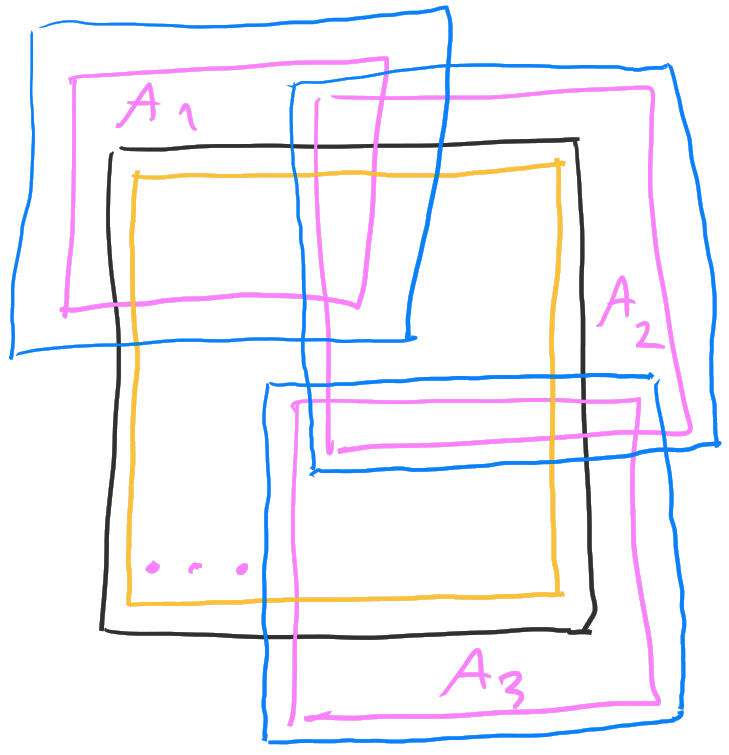
\includegraphics[width=.7\linewidth]{lect5_2.png}
        \caption{К утверждению \ref{lect5:cl4}.}
        \label{fig:lect5:2}
    \end{minipage}
\end{figure}

\begin{claim}
    \label{lect5:cl3}
    Клеточная мера~--- конечно-аддитивна.

    \begin{remark}
        Доказывалась в курсе матанализа, но идейно доказывается по индукции по числу клеток.
        Разрежем множество по какой-либо грани (смотри рисунок \ref{fig:lect5:1}). В силу выбора разреза, после него сверху и снизу число клеток
        уменьшится на один.
    \end{remark}
\end{claim}

\begin{claim}
    \label{lect5:cl4}
    Клеточная мера~--- $\sigma$"=аддитивна.

    \begin{proof}
        Докажем $\sigma$"=субаддитивность, тогда в силу утверждения \ref{lect5:cl2} получим $\sigma$"=аддитивность.

        Пусть $A\subset \bigcup\limits_{n=1}^{\infty}A_n$, где $A,\, A_n\in K_1$

        Во-первых, уменьшим клетку так, чтобы она стала компактом (на рисунке \ref{fig:lect5:2} это клетка оранжевого цвета):
        \[
            \forall\varepsilon>0\ \exists\text{замкнутая клетка } \widetilde{A}\subset A:\ m\left(\widetilde{A}\right)\geqslant m(A)-\varepsilon.
        \]

        Аналогично <<раздуем>> клетки $A_k$ так, чтобы клетки стали открытыми (синие клетки на рисунке):
        \[
            \forall n\in\N\ \exists\text{открытая клетка } \widetilde{A}_n\text{ такая, что } A_n\subset\widetilde{A}_n\text{ и }
            m\left(\widetilde{A}_n\right)\leqslant m(A_n)+\varepsilon_n,
        \]
        где $\varepsilon_n$ выберем позже.

        Тогда $\widetilde{A}\subset \bigcup\limits_{n=1}^{\infty}\widetilde{A_n}$, но $\widetilde{A}$~--- компакт, следовательно
        по лемме Гейне-Бореля существует конечное подпокрытие:
        \[
            \exists n_1,\,n_2,\,\ldots,\, n_l:\ \widetilde{A}\subset\bigcup_{i=1}^l\widetilde{A}_{n_l}\subset \bigcup_{n=1}^N \widehat{A}_n,
        \]
        где $N=\max(n_1,\,n_2,\,\ldots,\, n_l)$.
        В силу замечания после утверждения \ref{lect5:cl1} имеем:
        \[
            m(A)-\varepsilon\leqslant m(\widetilde{A})\leqslant\sum_{n=1}^Nm(\widetilde{A}_n)\leqslant\sum_{n=1}^{\infty}m(\widetilde{A}_n)
            \leqslant\sum_{n=1}^{\infty}m(A_n)+\leqslant\sum_{n=1}^{\infty}\varepsilon_n.
        \]
        Откуда окончательно,
        \[
            m(A)\leqslant \varepsilon+\sum_{n=1}^{\infty} m(A_n)+\sum_{n=1}^{\infty}\varepsilon_n\leqslant
            \sum_{n=1}^{\infty} m(A_n)+2\varepsilon,\text{ если } \varepsilon_n = \dfrac{\varepsilon}{2^n}.
        \]
        То есть, в силу того, что $\varepsilon$~--- произвольное, получаем требуемое:
        \[
            m(A)\leqslant \sum_{n=1}^{\infty} m(A_n).
        \]
    \end{proof}
\end{claim}